\documentclass[a0paper,landscape]{baposter}

\usepackage{lipsum}          % This is just for some blindtext

\usepackage{relsize}	       % For \smaller
\usepackage{url}			       % For \url
\usepackage{epstopdf}	       % Included EPS files automatically converted to PDF to include with pdflatex
\usepackage{multicol}        % Multi Columns
\usepackage{paralist} % For compact lists: compactitem

\usepackage{amsmath,amssymb} % math
\usepackage{natbib}
\usepackage{graphicx}
\usepackage{enumitem}

%%%%%%%%%%%%%%%%%%%%%%%%%%%%%%%%%%%%%%%%%%%%%%%%%%%%%%%%%%%%%%%%%%%%%%%%%%%%%%%%
%%% Utility functions %%%%%%%%%%%%%%%%%%%%%%%%%%%%%%%%%%%%%%%%%%%%%%%%%%%%%%%%%%
%%%%%%%%%%%%%%%%%%%%%%%%%%%%%%%%%%%%%%%%%%%%%%%%%%%%%%%%%%%%%%%%%%%%%%%%%%%%%%%%

%%% Save space in lists. Use this after the opening of the list %%%%%%%%%%%%%%%%
\renewcommand{\vec}[1]{\bm{#1}}
\newcommand{\vnabla}{\vec{\nabla}}

\renewcommand{\d}[1]{\text{d} #1}
\newcommand{\dxx}{\,\text{d}\vec{x}}
\newcommand{\dx}{\,\text{d}x}

\newcommand{\diff}[2]{\frac{\text{d}#1}{\text{d}#2}}
\newcommand{\idiff}[2]{\text{d}#1 / \text{d}#2}
\newcommand{\pdiff}[2]{\frac{\partial #1}{\partial #2}}
\newcommand{\pdifff}[2]{\frac{\partial^2 #1}{\partial #2^2}}
\newcommand{\ipdiff}[2]{\partial #1 / \partial #2}
\newcommand{\vdiff}[2]{\frac{\delta #1}{\delta #2}}
\newcommand{\ivdiff}[2]{\delta #1 / \delta #2}

%%%%%%%%%%%%%%%%%%%%%%%%%%%%%%%%%%%%%%%%%%%%%%%%%%%%%%%%%%%%%%%%%%%%%%%%%%%%%%%
%%% Document Start %%%%%%%%%%%%%%%%%%%%%%%%%%%%%%%%%%%%%%%%%%%%%%%%%%%%%%%%%%%%
%%%%%%%%%%%%%%%%%%%%%%%%%%%%%%%%%%%%%%%%%%%%%%%%%%%%%%%%%%%%%%%%%%%%%%%%%%%%%%%

\begin{document}
\typeout{Poster rendering started}

%%% General Poster Settings %%%%%%%%%%%%%%%%%%%%%%%%%%%%%%%%%%%%%%%%%%%%%%%%%%%
%%%%%% Eye Catcher, Title, Authors and University Images %%%%%%%%%%%%%%%%%%%%%%
\begin{poster}{
  columns=3,
	grid=false,
	borderColor=uniblue,
	headerColorOne=uniblue,
	headerColorTwo=uniblue,
	headerFontColor=white,
  headerheight=14em,
	boxColorOne=white,
  boxpadding=0.8em,
	headershape=rectangle,
	headerfont=\Large\textsf,
	textborder=none,
	background=shadetb,
  bgColorOne=white,
  bgColorTwo=white,
	headerborder=open,
  boxshade=plain,
  eyecatcher=false
}
%%% Eye Catcher %%%%%%%%%%%%%%%%%%%%%%%%%%%%%%%%%%%%%%%%%%%%%%%%%%%%%%%%%%%%%%%
{
}
%%% Title %%%%%%%%%%%%%%%%%%%%%%%%%%%%%%%%%%%%%%%%%%%%%%%%%%%%%%%%%%%%%%%%%%%%%
{diCtNN: A Dictionary-Enhanced CNN Approach \\ for Classifying Hate Speech on Twitter}
%%% Authors %%%%%%%%%%%%%%%%%%%%%%%%%%%%%%%%%%%%%%%%%%%%%%%%%%%%%%%%%%%%%%%%%%%
{
  \begin{multicols}{2}
  Carlos Eduardo Posada {\smaller (c.posada@mpp.hertie-school.org)\newline}
  Maximilian Kupi {\smaller (m.kupi@mpp.hertie-school.org)\newline}
  Michael Bodnar {\smaller (m.bodnar@mpp.hertie-school.org)\newline}
  Nikolas Schmidt {\smaller (n.schmidt@mpp.hertie-school.org)}
  \end{multicols}
}
%%% Logo %%%%%%%%%%%%%%%%%%%%%%%%%%%%%%%%%%%%%%%%%%%%%%%%%%%%%%%%%%%%%%%%%%%%%%
{\begin{minipage}{30.0em}
    
\includegraphics[width=30.0em]{hertie}
  \end{minipage}
}

%%% Box 1 %%%%%%%%%%%%%%%%%%%%%%%%%%%%%%%%%%%%%%%%%%%%%%%%%%%%%%%%%%%%%%%%%%
\headerbox{Problem}{name=abstract,column=0,row=0}{
\begin{center}
\begin{compactitem} 
    \item \textbf{Hate speech targets} individuals or groups based on identity, and may influence the occurrence of hate crimes.
    \item \textbf{Social media} can serve as a propagation mechanism.
    \item \textbf{Necessity of automatic removal} of hateful comments from social media.
    \item \textbf{Deep learning methods} are effective.
    \item \textbf{Limitation}: Hate speech is hard to define, elusive and evolving. Negative sentiment $\neq$ hate speech. Offensive content $\neq$ hate speech.
    \item \textbf{Ambition:} Adaptability and data minimisation: Detect hateful content (in text - versatile), not hateful users (in metadata - platform-specific). 
    \item \textbf{Our proposal}: \textit{diCtNN, a deep-learning classifier of hate speech in tweets (adaptable to text classification in other domains).}
    \begin{compactitem}
        \item Convolutional Neural Network (CNN)
        \item Three-class classification: "hateful", "abusive", "normal"
        \item Dictionary approach
    \end{compactitem}
\end{compactitem}
\end{center}
}

%%% Box 2 %%%%%%%%%%%%%%%%%%%%%%%%%%%%%%%%%%%%%%%%%%%%%%%%%%%%%%%%%%%%%%%%%%%%%

\headerbox{Data/Task}{name=task,column=0,below=abstract}{
\begin{compactitem}
    \item \textbf{Dataset:} 110,638 tweets (merged from two datasets \cite{hateoffensive} \& \cite{founta2018large})
 \end{compactitem}
\begin{center}

\includegraphics[width=0.9\textwidth]{figures/faketweet_poster.pdf}
\textit{Example Tweet. Note: Graphic language for illustration purposes.}
\end{center}
\begin{compactitem}
    \item \textbf{Three-class classification:} Hateful ($0$) - Abusive ($1$) - Normal ($2$)
    \item \textbf{Deep Learning Classifier:} Convolutional Neural Network (CNN)
    \item \textbf{Baseline:} 1D-architecture; \textit{Input:} Tensor of BERT-vectorised tweets
    \item \textbf{Enhanced model}: 2D-architecture; \textit{Input:} Matrix of stacked tensor: Tensor of BERT-vectorised tweets \& Tensor containing measure of hatefulness in tweet, stacked
 \end{compactitem} 
}

%%% Box 3 %%%%%%%%%%%%%%%%%%%%%%%%%%%%%%%%%%%%%%%%%%%%%%%%%%%%%%%%%%%%%%%%%%%%%
\headerbox{Proposed Method}{name=method,column=1}{
\begin{enumerate} 
    %Describe your main methods/techniques/models. Diagrams are generally better than text, and equations should be used sparingly (if at all). Highlight the core idea of your techniques.
    \item \textbf{Preprocessing:} Noise removal: lower-casing, symbols, whitespaces, standalone digits and tweet-specific traits).
    \item \textbf{Vectorisation process}
\end{enumerate}
\begin{center}
    %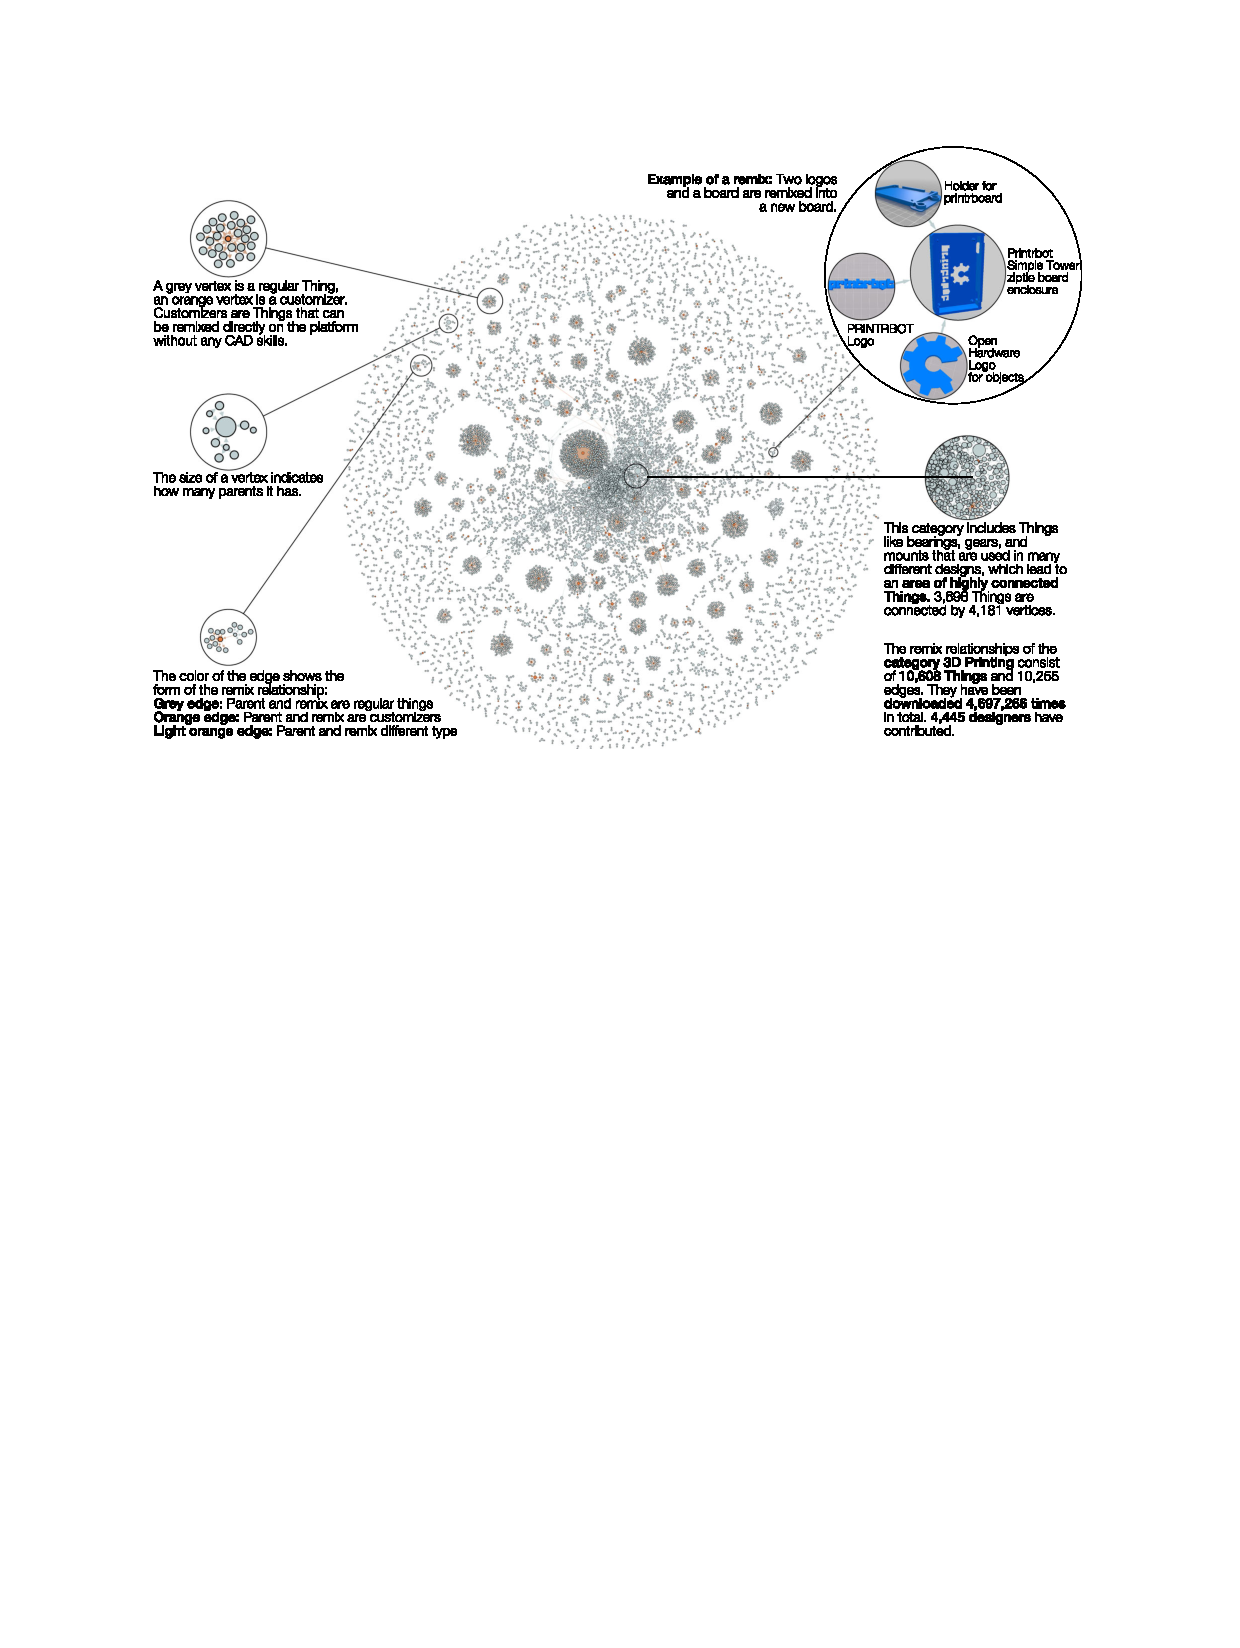
\includegraphics[width=0.9\textwidth]{ctc.pdf}
    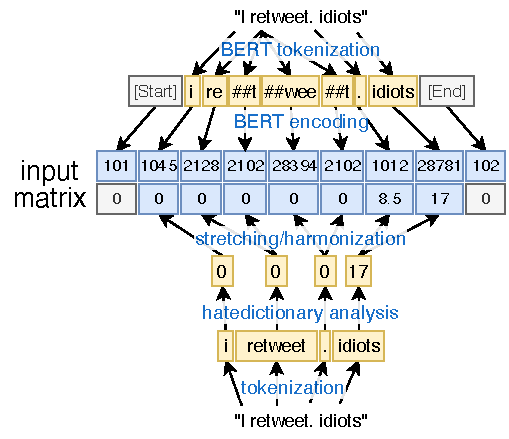
\includegraphics[scale=1.2]{figures/processing-regular.pdf}
\end{center}
}

%%% Box 4 %%%%%%%%%%%%%%%%%%%%%%%%%%%%%%%%%%%%%%%%%%%%%%%%%%%%%%%%%%%%%%%%%%%%%
\headerbox{Results}{name=results,column=1,below=method}{

    %Present your most important results. Tables containing many numbers are overwhelming. Be selective and choose just the results that convey the story you’re telling. Make it clear what the evaluation metrics are, and what’s being compared.
\textbf{Best model (grid search):}\
\textit{Optimizer:} Adam - \textit{Learning rate:} 0.01 - \textit{Scheduler:} Deactivate - \textit{Loss function:} Containing class weights // \textbf{Epoch:} 29 (1D) - 36 (2D) // \textbf{Improvement from 1D to 2D:} \textit{Accuracy:} 6 pp - \textit{F1 Macro}: 7 pp 
\begin{center}
    \begin{tabular}{c}
    2D Model with diCtNN Preprocessing \\
    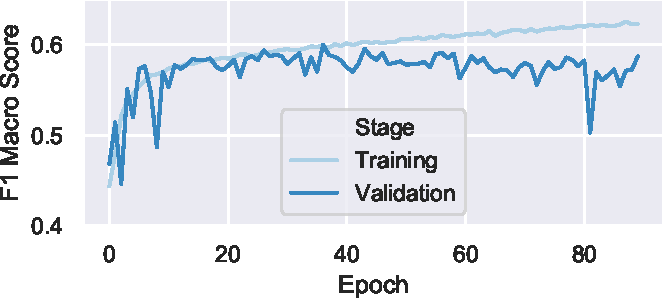
\includegraphics[width=8cm, keepaspectratio]{figures/f1_diCtNN_Model_27_90epochs_wp.pdf}
    \end{tabular}
\end{center}
}

%%% Box 5 %%%%%%%%%%%%%%%%%%%%%%%%%%%%%%%%%%%%%%%%%%%%%%%%%%%%%%%%%%%%%%%%%%%%%
\headerbox{Analysis}{name=analysis,column=2}{
    \begin{compactitem}
        \item \textbf{Precision and recall increase $\uparrow$:} diCtNN distinguishes between hate, abusive and normal speech on Twitter \textit{better} than baseline.
    \end{compactitem}

   % Show any plots, diagrams, examples and visualisations to provide interesting analysis. Make it clear what the reader should conclude from each figure.
\begin{center}
    \begin{tabular}{c}
    1D Model with BERT Preprocessing \\
    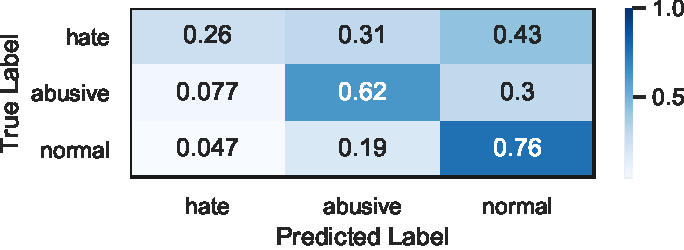
\includegraphics[width=8cm,keepaspectratio]{figures/confusion_matrix_testing_CNN_experiment_1D_FINAL.pdf} \\
    \\
    2D Model with diCtNN Preprocessing \\
    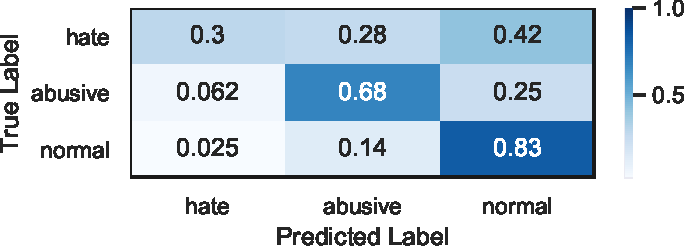
\includegraphics[width=8cm,keepaspectratio]{figures/confusion_matrix_testing_CNN_experiment_2D_FINAL.pdf}
    \end{tabular}
\\
    \begin{compactitem}
    \item \textbf{False negatives remain} due to: 
    1. Class imbalance // \newline 2. Wrong manual labelling // 3. Difficulties finding hateful terms // 4. Imperfect hate speech dictionary and definition.
    \end{compactitem}
\end{center}
}

%%% Box 6 %%%%%%%%%%%%%%%%%%%%%%%%%%%%%%%%%%%%%%%%%%%%%%%%%%%%%%%%%%%%%%%%%%%%%
\headerbox{Conclusions}{name=conclusions,column=2, below=analysis}{
\begin{compactitem}
    \item \textbf{diCtNN works well} on \textit{hate speech classification}. It can be \textit{adapted to other text classification problems,} if there's a similar dictionary.
    \item \textbf{ToDo:} Use model on \textit{other datasets and compare it to establish baselines}. Try out \textit{other DL architectures}. Vet and regularly update dictionary in case of \textit{deployment for live hate speech detection}.
\end{compactitem}
}

%%% Box 7 %%%%%%%%%%%%%%%%%%%%%%%%%%%%%%%%%%%%%%%%%%%%%%%%%%%%%%%%%%%%%%%%%%%%%
\headerbox{References}{name=references,column=2,below=conclusions, above=bottom}{

\begingroup
\renewcommand{\section}[2]{}%
%\renewcommand{\chapter}[2]{}% for other classes
{\small
\bibliographystyle{chicago}
\bibliography{references.bib}
}
\endgroup
}

\end{poster}
\end{document}